Parental controls are typically marketed with generic claims about their functionalities, promising to protect children while providing no information about their functioning.
To investigate their actual implementations and effectiveness, we examined the consumer market for parental control solutions across hardware, software and the DNS. 
% We compiled a list of parental controls solutions from routers with integrated parental control features and software products to test on Windows devices.
% \todo[inline]{They could ask why we did not include \st{DNS}, ISPs and browsers in this point. Anna: indeed. We need to add a sentence in RW about considering ISP and browsers out of scope}
To try and ensure broad coverage and relevance we aimed to identify devices and services that are likely to be adopted by actual families. 
Our selection was guided by three criteria:

\begin{enumerate}
\item Popularity, which we determined trough user reviews and ratings (considering both the amount of reviews and the score) on retail platforms such as Amazon. 
\item  Market relevance, recognized from mentions in consumer-focused rankings (e.g. blog-posts about the best parental controls of the year on technology forums) and professional reviews.
\item Diversification, aiming to include major providers to reflect the available commercial offerings, rather than focusing on a single vendors solutions.
\end{enumerate}

%\begin{table*}[!t]
 %   \centering
  %  \begin{tabular}{|c|c|}
   % \hline
    % \textbf{Solution} & \textbf{Type} \\
     %\hline
     %TP-Link (Archer AX10) & Router \\
     %\hline
     %Netgear (Nighthawk series ADD EXACT MODEL) & Router \\
     %\hline
     %ASUS (RT-AX56U) & Router \\
     %\hline
     %Norton Family & Software \\
     %\hline
     %OpenDNS FamilyShield & DNS \\
     %\hline
     %DNS.eu & DNS \\
     %\hline
    %\end{tabular}
    %\caption{Parental control solutions considered in the study}
    %\label{tab:parental_controls}
%\end{table*}


From this process, we selected three router solutions, one software solution and two DNS-based filtering mechanisms, which are summarized in Table~\ref{tab:parental_controls}.

\begin{table}[htbp]
	\centering
    \begin{tabular}{|c|c|}
    \hline
    \textbf{Solution} & \textbf{Type} \\
    \hline
    TP-Link (Archer AC1900) & Router \\
    \hline
    Netgear (Nighthawk AX5400) & Router \\
    \hline
    ASUS (RT-AX57) & Router \\
    \hline
    Norton Family & Software \\
    \hline
    OpenDNS FamilyShield & DNS \\
    \hline
    DNS.eu & DNS \\
    \hline
    \end{tabular}
    \vspace{0.5\baselineskip} 
    \caption{Parental control solutions analyzed in the study}
    \label{tab:parental_controls}
\end{table}
    
    

% From this process, we selected three routers from three different manufacturers: TP-Link (Archer AX10), Netgear (Nighthawk series ADD EXACT MODEL), and ASUS (RT-AX56U).
% On the software side trough the same process we selected Norton Family.
%\todo[inline]{Anna: Check the commented paragraph in here, some of the text can be used in the RW.}
% While our initial focus was on hardware-based parental controls, early tests on the ASUS router revealed that its filtering mechanism relied on external DNS services.
% Based on this observation, we decide to extend our analysis to include examples of DNS-based parental control services, which apply filtering at the resolver level.
% As a result, we added OpenDNS FamilyShield and DNS.eu Kids to our evaluation.
% These resolvers are commonly used in private, professional or institutional networks to restrict access to inappropriate or dangerous websites.
% Their inclusion allowed us to compare router-level filtering with dedicated DNS services, using the same Tranco domain list.

%\todo[inline]{Anna: we need to check if we want to keep this here or if we want to have a separate subsection.}
To evaluate how each parental control system handles different types of content, we 
designed our tests around a popularity list of domains (see Sec.~\ref{sec:dataset}) and the set of identified parental control solutions. To identify which domains should be blocked by a parental control, we rely on content categories, such as porn and gambling, using domain classification data (see Sec.~\ref{sec:dataset}).
In particular, we tested how each solution blocks or allows each of the domains in the popularity list. Since we expected the selected solutions to have different blocking methodologies (e.g. DNS or HTTPS), we used different approaches targeting the specific solutions. We therefore first define a behaviour baseline for each solution (See ~\ref{sec:results-baseline}).

%  list derived from the Tranco dataset\footnote{\url{https://tranco-list.eu/}}.
% Tranco aggregates the most visited websites across multiple popularity rankings (including Cisco Umbrella, and Majestic), and provides the top 1M popular domains list updated daily.
% This dataset forms the basis of our tests, enabling us to analyze filtering behavior across a wide range of websites.
% Within the Tranco dataset, we identified content inappropriate for minors (e.g., pornography, gambling) using the classification provided by Cisco Umbrella. 
% (add link and short explanation of what Cisco did)
% A more detailed discussion of this classification process appears in Sec.~\ref{sec:dataset}.

Each of the identified solutions necessitates of a specific data collection methodology, which we explain in the following subsections.


\subsection{Routers}
To analyze how each router implements its parental control functionalities, we built a controlled environment involving three physical routers and three dedicated client PCs. Each PC is connected via LAN to one router.
Each router is connected to the Internet via its WAN port, allowing it to resolve DNS queries and apply filtering policies as it would in a real-world scenario.
To capture and analyze traffic, we tapped both the LAN and WAN connections:
The LAN capture records the traffic sent by the client PC to the router and the router's responses.
The WAN capture monitors traffic between the router and the Internet, including DNS lookups and connections to web servers.

\begin{figure}[htbp]
    \centering
    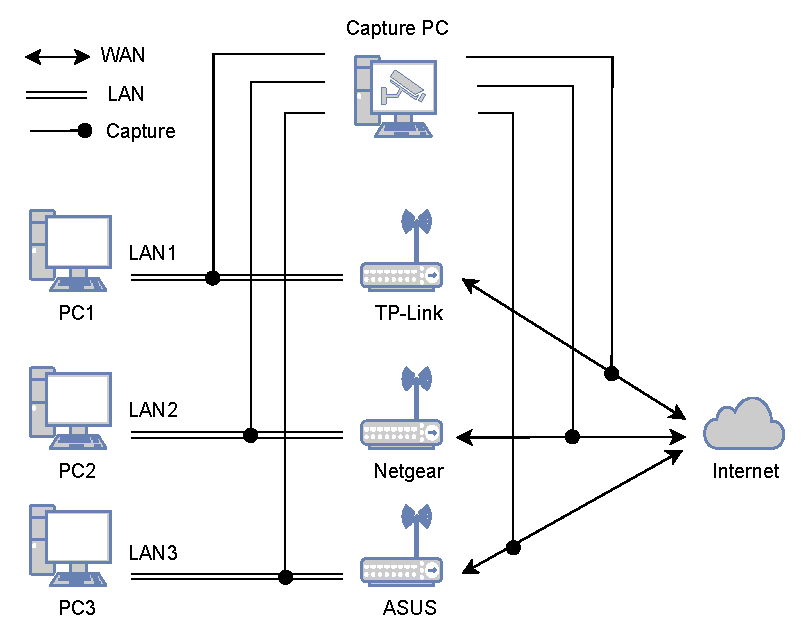
\includegraphics[width=0.9\linewidth]{Images/Methodology/capture.pdf}
    \caption{Capture setup to investigate the behaviour of the routers.}
    \label{fig:capture}
\end{figure}

This setup, shown in Figure~\ref{fig:capture}, gives us an overview of the traffic entering and exiting each router. 
We captured PCAPs of each connection and used Wireshark to analyze them and extract information about the behaviour of the routers.
By comparing what is sent by the PC and what is allowed to leave (or blocked) by the router, we can observe exactly how each device enforces its parental control policies, especially at the DNS level.
%On the computer, these tunnels are linked to different virtual networks (VLANs), each one assigned to a specific port on a switch.
%Each of those switch ports is connected to the WAN port of a different router (TP-Link, Netgear, ASUS).
%With this setup the VM can send traffic directly to each router as if it were a regular Internet connection.
%At the same time, each router’s LAN port is connected back to the switch on another set of ports. 
%These ports use different VLANs, and the desktop sends that traffic back through tunnels to the same VM. 
%This way, the VM sees both the traffic toward the router (trough the WAN) and what comes out of it (trough the LAN), letting us monitor how the router modifies each request.
% This setup lets us automate the testing of the routers parental control functionalities while keeping the communications under control.
Each router was tested with parental controls enabled and disabled, allowing us to isolate and understand the specific blocking behavior.
% We initially ran the tests with full HTTP/HTTPS browsing, but we realized that the resulting PCAPs were too large for scalable analysis.
% We then developed a lightweight testing script that performs only DNS lookups (via a --noHttp flag), greatly reducing traffic volume while still capturing blocking behavior.

\subsubsection{The TP-Link case}
The TP-Link router uses a set of user-defined keywords as base for its filtering mechanisms. This implies that we need to initialize such a set before conducting our experiments. In this case, we tried to put ourselves in the shoes of a parent confronted with such a task, and we therefore asked ChatGPT to create a list of keywords (31 words, as this is the maximum allowed by TP-Link), based on a set of website categories of inappropriate or harmful content (see Sec.~\ref{sec:dataset}).

\subsection{Software}
For software-level parental controls, we analyzed Norton Family. 
We installed the software solution on a Windows machine. We iterate over the input list of domains using a curl script and we monitored the outgoing traffic using Wireshark to collect possible evidence of blocking behaviour.  

%ANTONIA move to results
% Our initial approach was similar to the one used for the routers, capturing PCAPs using Wireshark during browsing sessions. 
% However, Norton was not suited for this type of measurement. 
% We observed inconsistent signs of activity, such as failed TLS handshakes, or unexplained delays. 
% These artifacts were not regular or reliable enough to support a large scale measurement.
% For this reason, we developed an alternative detection strategy.
% After exploring several approaches, including monitoring the behavior of the browser extensions installed by Norton, we settled on a curl-based script.
% This script visits each domain and determines whether it is blocked by analyzing the resulting HTML content.
%Specifically, the script looks for known indicators of a Norton block page, such as the presence of the word “NortonLifeLock” and references to the logo file used in the block page.

% Mobicip functions as a \st{certification authority} transparent proxy, installing its own root certificate and intercepting all HTTPS traffic at the local device level.
% To reliably detect which domains were being blocked, we developed an automated testing script using Playwright (https://playwright.dev/), an open-source tool for controlling browsers.
% We used it to run a headless browser, meaning a browser that operates without a visible user interface, 
% This approach is good for large-scale automated testing since it consumes fewer resources and has faster execution time, compared to a full browser session.
 
\subsection{DNS}
% {WE ALREADY EXPLAINED WHY WE ADDED THESE SERVICES, SHOULD I ADD MORE AS AN INTRODUCTION. Anna: no I think this is enough at the moment
% descritto separatamente va bene (e.g. nella subsection DNS), ma nell'introduzione e nella parte introduttiva della metodologia direi semplicemente quello che abbiamo scelto, non come ci siamo arrivati}
OpenDNS FamilyShield and DNS.eu Kids are publicly accessible DNS resolvers that advertise family-safe filtering.
To analyze their behavior, we created a measurement script that uses the dig to send DNS queries to each service.
%The script records the DNS response and classifies a domain as blocked if the response is empty (for DNS.eu Kids) or it contains a known block IP (\texttt{146.112.61.106} for OpenDNS).
We limited the number of daily queries sent to each service to prevent rate-limiting or automatic blocking.


